\documentclass[crop,tikz]{standalone}

\tikzset{>=latex}

\begin{document}
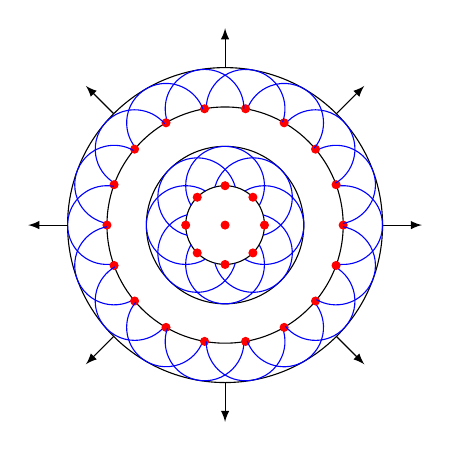
\begin{tikzpicture}
  \foreach \R in {0.5,1,1.5,2} { \draw (0,0) circle (\R); }
  \foreach \R in {0.5} {%
    \foreach \A in {0,45,...,315} {%
      \draw[blue] (\A:\R)+(\A-120:0.5) arc (\A-120:\A+120:0.5);
      \draw[fill,red] (\A:\R) circle (0.05);
    }
  }
  \foreach \R in {1.5} {%
    \foreach \A in {0,20,...,340} {%
      \draw[blue] (\A:\R)+(\A-100:0.5) arc (\A-100:\A+100:0.5);
      \draw[fill,red] (\A:\R) circle (0.05);
    }
  }
  \foreach \X in {0,45,...,315} { \draw[->] (\X:2) -- +(\X:0.5); }
  \draw[fill,red] (0,0) circle (0.05);
\end{tikzpicture}
\end{document}
